%!TEX root = Manuscript.tex

\chapter{Applications and Datasets}
\label{chap:ApplicationsAndDatasets}
%Before revealing the details of the rough-to-precise matching strategy, 
In this section, five sets of datasets categorized in four application scenarios are introduced (cf. Table ~\ref{application}), which will be used to test our pipeline.

\begin{table}[htbp]
	%\scriptsize %\footnotesize
	\centering
	\begin{tabular}{||l|l||c||}\hline
		 \multicolumn{2}{||c||}{Application scenario} & Dataset \\\hline\hline
		 \multirow{2}{*}{General case for change detection} & Urban area & Fr{\'e}jus \\
		 & Rural area & Pezenas \\\hline
		 \multicolumn{2}{||c||}{Earthquake case} & Kobe \\\hline
		 \multicolumn{2}{||c||}{Landslide case} & Alberona \\\hline
		 \multicolumn{2}{||c||}{Glacier case} & Hofsjökull \\\hline
	\end{tabular}
	\caption{Five sets of datasets categorized in four application scenarios.}
	\label{application}
\end{table}

Details of the datasets are listed in Table~\ref{AerialData}, ~\ref{SatelliteData}. 
Images demonstrations of each dataset are displayed in Figure~\ref{FrejusData},~\ref{PezenasData}, ~\ref{KobeData}, ~\ref{AlberonaData} and ~\ref{Hofsjökull}.

%General case for change detection
%	Rural area: Pezenas
%	Urban area: Fr{\'e}jus
%Earthquake case: Kobe
%Landslide case: Alberona
%Glacier case: Hofsjökull

\section{General case for change detection}
%Two sets of datasets are chosen to 
\subsection{Urban area: Fr{\'e}jus}
The dataset Fr{\'e}jus is an urban area, mainly covered with buildings along with scattered farmlands, except a half-moon-shaped bay located in south. It is a 15 $km^2$ rectangular area located in Fr{\'e}jus, a commune in southeastern France. We have four sets of aerial images acquired in 1954, 1966, 1970 and 2014. The epoch 2014 was acquired with the \ac{IGN}'s digital metric camera ~\cite{souchon2010ign}, its orientations are both in global reference frame and precise. Therefore it is treated as \ac{GT} during our processing (in other words, their parameters will be fixed during the \ac{BBA}). 
The area exhibits drastic scene changes in the 60-year period, as can be seen in Figure~\ref{FrejusEvolution}, where evolution of a subregion is displayed.\\

\subsection{Rural area: Pezenas}
The dataset Pezenas is a rural area, mainly covered with vegetation and several sparsely populated urban zones. It is a 420 $km^2$ rectangular area located in Pezenas in the Occitanie region in southern France. We have at our disposal three sets of aerial images acquired in 1971, 1981 and 2015, and one set of satellite images acquired in 2014. Both the epoch 2014 and 2015 are treated as \ac{GT}. In this dataset we are interested in matching historical epochs (1971 and 1981) with aerial \ac{GT} and satellite \ac{GT} individually. The area exhibits changes in scene appearance in the 44-year period.\\

\section{Earthquake case: Kobe}
The dataset Kobe witnessed the well-known Kobe earthquake in January 1995. It is a 90 $km^2$ area of irregular shape located in the north of Awaji Island, Japan. We have two sets of aerial images: pre-event acquired in 1991 and post-event acquired in 1995. It is mainly covered with mountain area and narrow urban zones along the sea. There are neither \ac{GT} epochs nor \ac{GCP}s, therefore we measured 2 points on Google map to scale the result to metric units. In this dataset we are interested in localizing the earthquake fault.

\section{Landslide case: Alberona}
The dataset Alberona is characterized by the diffuse presence of clay rich lithologies which confers to the landscape a typical smooth topography, with the wide presence of slow moving landslides of the slide and slide-earthflow type. It is a 90 $km^2$ rectangular area located in Southern Italy, near the village of Alberona (Puglia region). 
In the study area, the land use is typical of rural areas, poorly inhabited and mainly agricultural and wooded. A slow moving slide-earthflow has been detected there since the 1950s. 
Images were scanned with non photogrammetric scanner with 800 dpi. The films were poorly preserved before scanning, which present some scratches and dust, a typical feature for images that were not preserved for photogrammetric purposes.
There are no \ac{GT} epochs but 7 \ac{GCP}s which could be used to move the results in relative coordinate systems to the absolute one.
In this dataset we are interested in localizing the landslide.

\section{Glacier case: Hofsjökull}
The dataset Hofsjökull is a snow-covered area located in Hofsjökull in central Iceland. Unlike other datasets discribed previously, Hofsjökull consists of only one epoch, as in this dataset we are only interested in matching challenging intra-epoch image pairs. It contains several archival aerial images acquired in the year 1960, provided by the National Survey of Iceland. They were scanned with a photogrammetric scanner Wehrli RM-6, in 16micron/px and 12 bit, in order to digitize as much information as possible appearing in the films. In Figure~\ref{Hofsjökull} we displayed 6 consecutive images in the same flight strip, with snow-covered area gradually expanding. The most challenging image pair (i.e. image 5 and 6, as they are fully snow-covered with very limited context) are chosen for testing. Their common zone is labeled with red rectangles. 

\begin{table}[htbp]
	\scriptsize %\footnotesize
	\centering
	\begin{tabular}{||c|c||c|c|c|c|c|c|c|c|c||}\hline
& \multirow{2}{*}{Epoch} & F & Wid & Hei & GSD & \multirow{2}{*}{F. o.} & \multirow{2}{*}{S. o.} & H & \multirow{2}{*}{Nb} & \multirow{2}{*}{Flightline} \\
&  & [pix] & [mm] & [mm] & [m] & & & [m] & & \\\hline\hline

\multirow{4}{*}{Fr{\'e}jus} & 1954 & 23350 & 300 & 300 & \color{black}0.11 & 60\% & 20\% & 2500 & 19 & West-Est \\
& 1966 & 10230 & 180 & 180 & \color{black}0.17 & 60\% & 30\% & 1700 & 15& West-Est \\
& 1970 & 10230 & 180 & 180 & 0.17 & 60\% & 30\% & 1700 & 19& West-Est \\
& 2014 & \color{black}18281 & 99.28 & 72.42 & 0.35 & 60\% & 30\% & 6500 & 33& West-Est \\\hline\hline

\multirow{4}{*}{Pezenas} & 1971 & 7589 & 230 & 230 & 0.32 &    60\% &    20\% & 2400 & 57& West-Est \\
& 1981 & 7607 & 230 & 230 & 0.59 & 60\% & 20\% & 4500 & 27& West-Est \\
& \multirow{2}{*}{E2015} & 9967.5 & 47 & 35 & 0.46 & 60\% & 50\% & 4600 & 308& West-Est \\
&  & 9204.5 & 50 & 36 & 0.5 & 60\% & 50\% & 4600 & 74& West-Est \\\hline\hline

\multirow{2}{*}{Kobe}& 1991& 7662 & 212 & 212 & 0.5 &    65\% &    35\% & 3800 & 15 & Northeast-Southwest \\
& 1995& 7662 & 212 & 212 & 0.18 & 65\% & 65\% & 1400 & 83& Northeast-Southwest \\\hline\hline

\multirow{2}{*}{Alberona}& 1954 & 4760 & 230 & 230 & 1.0 & 65\% & / & 6000 & 3& North-South \\
& 2003 & 4650 & 230 & 230 & 0.85 & 65\% & 30\% & 4850 & 7 & West-Est \\\hline\hline

Hofsjökull & 1960 & 9656 & 224 & 224 & 0.57 & 60\% & / & 5480 & 6 & North-South \\\hline
	\end{tabular}
	\caption{Aerial dataset details of Fr{\'e}jus, Pezenas, Kobe, Alberona and Hofsjökull. The 2015 acquisition of Pezenas is obtained with two sets of camera. F means focal length, Wid and Hei are the width and height of image, GSD is the ground sampling distance, F.o. and S.o. are forward and side overlap, H is the flying height, Nb is the number of images.}
	\label{AerialData}
\end{table}

%\begin{table}[htbp]
%    \scriptsize %\footnotesize
%    \centering
%    \begin{tabular}{||l|c|c|c|c||c|c|c|c||c|c||}\hline
%        &\multicolumn{4}{c||}{Fr{\'e}jus}&\multicolumn{4}{c||}{Pezenas}&\multicolumn{2}{c||}{Kobe}\\\hline
%                &E1954&E1966&E1970&E2014&E1971&E1981&\multicolumn{2}{c||}{E2015}&E1991&E1995\\\hline\hline
%        F [pix]&23350&10230&10230&\color{black}18281&7589&7607&9967.5&9204.5&7662&7662\\
%        %Size [mm]&\color{black}300,300&\color{black}180,180&\color{black}180,180&99.28,72.42&230230&230230&47,35&50,36&212212&212,212\\
%        Wid [mm]&300&180&180&99.28&230&230&47&50&212&212\\
%        Hei [mm]&300&180&180&72.42&230&230&35&36&212&212\\
%        GSD [m]&\color{black}0.11&\color{black}0.17&0.17&0.35&0.32&0.59&0.46&0.5&0.5&0.18\\
%        F. o.&60\%&60\%&60\%&60\%&   60\%&60\%&60\%&60\%&   65\%&65\%\\
%        S. o.&20\%&30\%&30\%&30\%&   20\%&20\%&50\%&50\%&   35\%&65\%\\
%        H  [m]&2500&1700&1700&6500&2400&4500&4600&4600&3800&1400\\
%        Nb &19&15&19&33&57&27&308&74&15&83\\\hline
%    \end{tabular}
%    \caption{Aerial dataset details of Fr{\'e}jus, Pezenas and Kobe. The 2015 acquisition of Pezenas is obtained with two sets of camera. E stands for epoch, F means focal length, Wid and Hei are the width and height of image, GSD is the ground sampling distance, F.o. and S.o. are forward and side overlap, H is the flying height, Nb is the number of images.}
%    \label{AerialData}
%\end{table}

\begin{table}[htbp]
	\scriptsize %\footnotesize
	\centering
	\begin{tabular}{||l|c|c||}\hline
		& Master image & Secondary image\\\hline
		Constellation & Pleiades & Pleiades \\
		GSD [m] & 0.5 & 0.5\\
		Acquired date & 12/06/2014 & 12/06/2014 \\
		Number of lines & 38468 & 37710 \\
		Number of pixels per line & 34108 & 33392 \\
		Cloud cover & 3.9\% & 4.0\% \\
		Snow cover & 0\% & 0\% \\\hline
		%B/H?
	\end{tabular}
	\caption{Satellite dataset details of Pezenas. GSD means the ground sampling distance.}
	\label{SatelliteData}
\end{table}

\begin{figure*}[htbp]
    \begin{center}
        \subfigure[Fr{\'e}jus 1954 (19 images)]{
            \begin{minipage}[t]{0.4\linewidth}
                \centering
                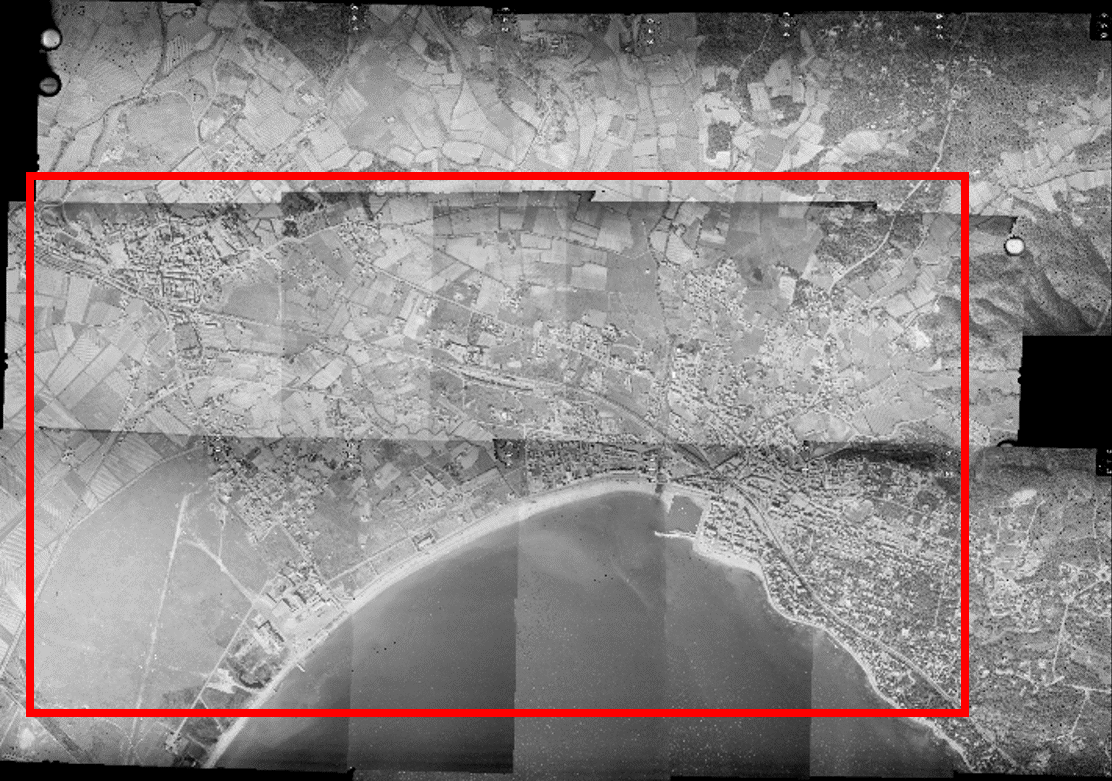
\includegraphics[width=5.65cm]{images/Chapitre3/Frejus1954.png}
            \end{minipage}%
        }
        \subfigure[Fr{\'e}jus 1966 (15 images)]{
            \begin{minipage}[t]{0.56\linewidth}
                \centering
                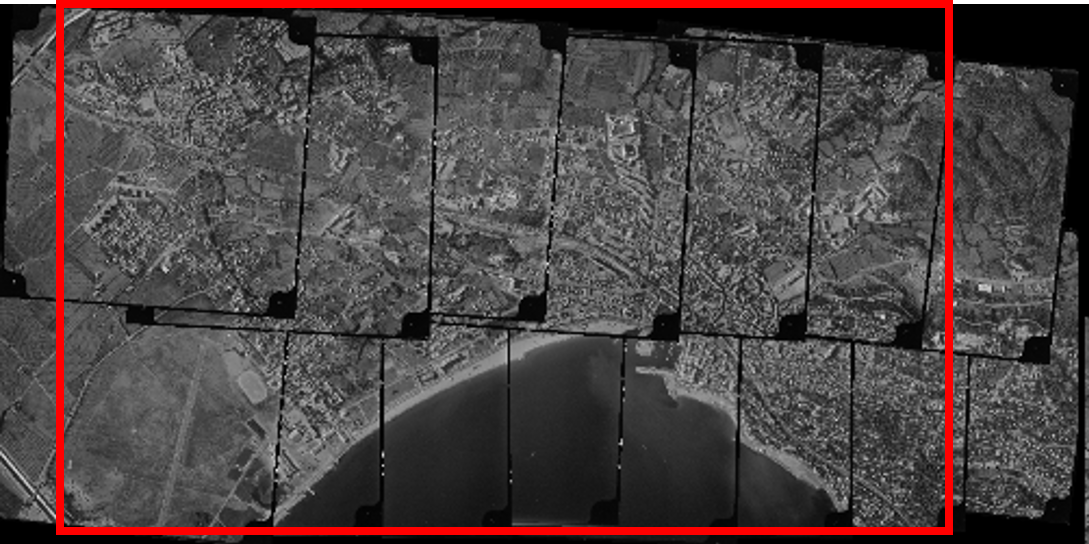
\includegraphics[width=7.6cm]{images/Chapitre3/Frejus1966.png}
            \end{minipage}%
        }
        \subfigure[Fr{\'e}jus 1970 (19 images)]{
    \begin{minipage}[t]{0.5\linewidth}
        \centering
        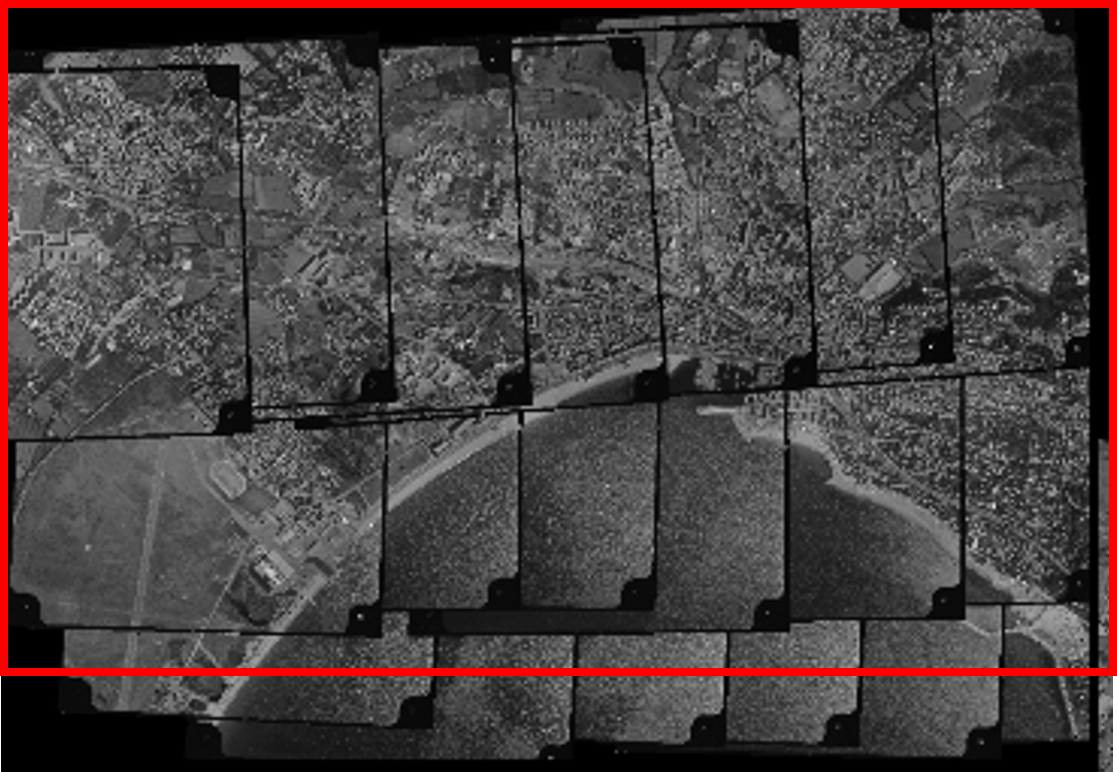
\includegraphics[width=6.1cm]{images/Chapitre3/Frejus1970.png}
    \end{minipage}%
}
\subfigure[Fr{\'e}jus 2014 (36 images)]{
    \begin{minipage}[t]{0.46\linewidth}
        \centering
        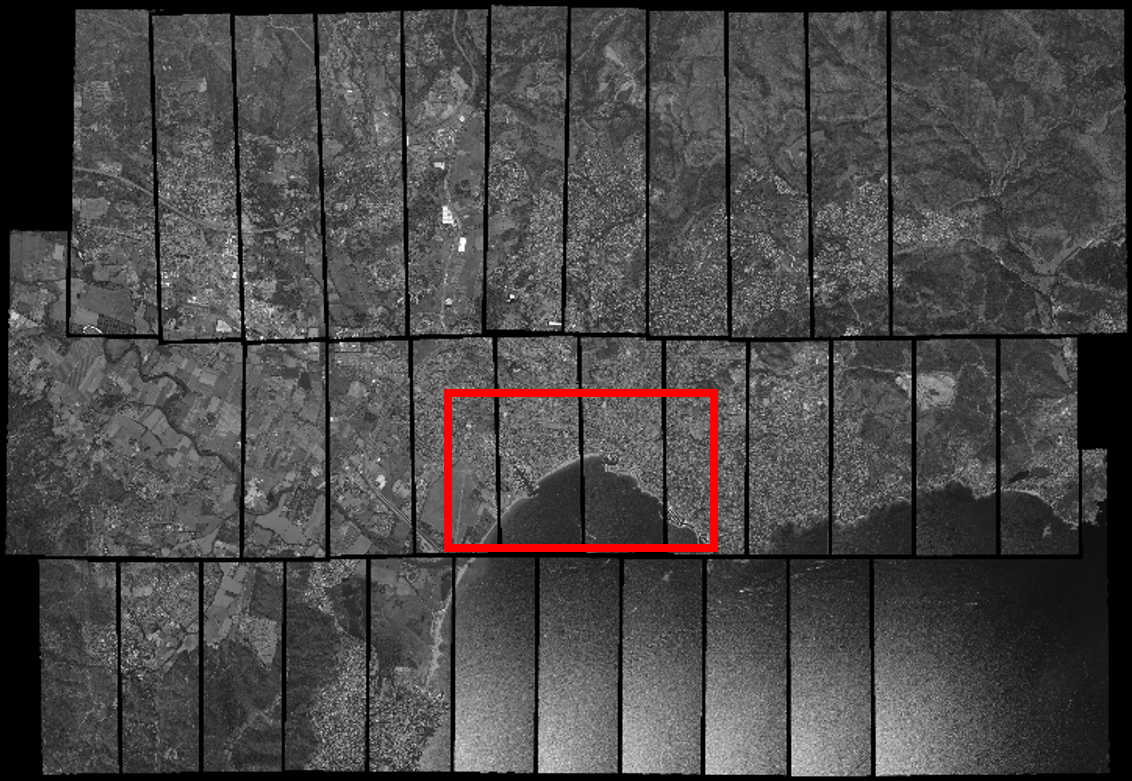
\includegraphics[width=6.25cm]{images/Chapitre3/Frejus2014.png}
    \end{minipage}%
}
        \caption{Images demonstration of different aerial epochs in \textbf{Fr{\'e}jus}, image number of each epoch is displayed in the parenthesis of each sub headline. The common zone between all the epochs is indicated by the red rectangles. Graphic scale is demonstrated on epoch 2014 in (d).}
        \label{FrejusData}
    \end{center}
\end{figure*} 

\begin{figure*}[htbp]
	\begin{center}
		\subfigure[Subregion of Fr{\'e}jus 1954]{
			\begin{minipage}[t]{1\linewidth}
				\centering
				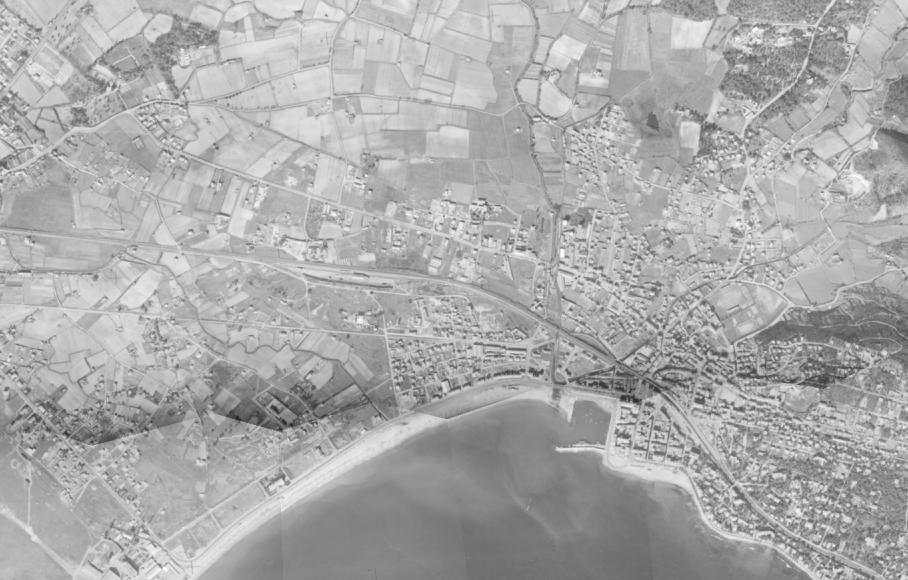
\includegraphics[width=13cm]{images/Chapitre3/Frejus1954Sub.png}
			\end{minipage}%
		}
		\subfigure[Subregion of Fr{\'e}jus 2014]{
			\begin{minipage}[t]{1\linewidth}
				\centering
				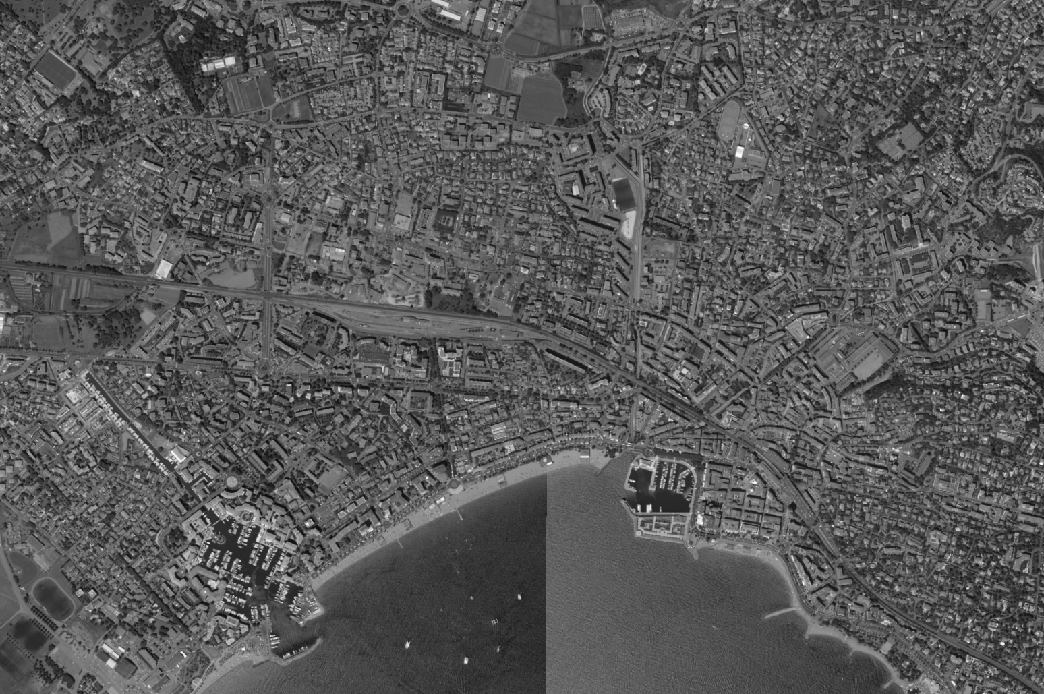
\includegraphics[width=13cm]{images/Chapitre3/Frejus2014Sub.png}
			\end{minipage}%
		}
		\caption{Evolution of a subregion in Fr{\'e}jus.}
		\label{FrejusEvolution}
	\end{center}
\end{figure*} 

\begin{figure*}[htbp]
    \begin{center}
        \subfigure[Pezenas 1971 (57 images)]{
            \begin{minipage}[t]{0.48\linewidth}
                \centering
                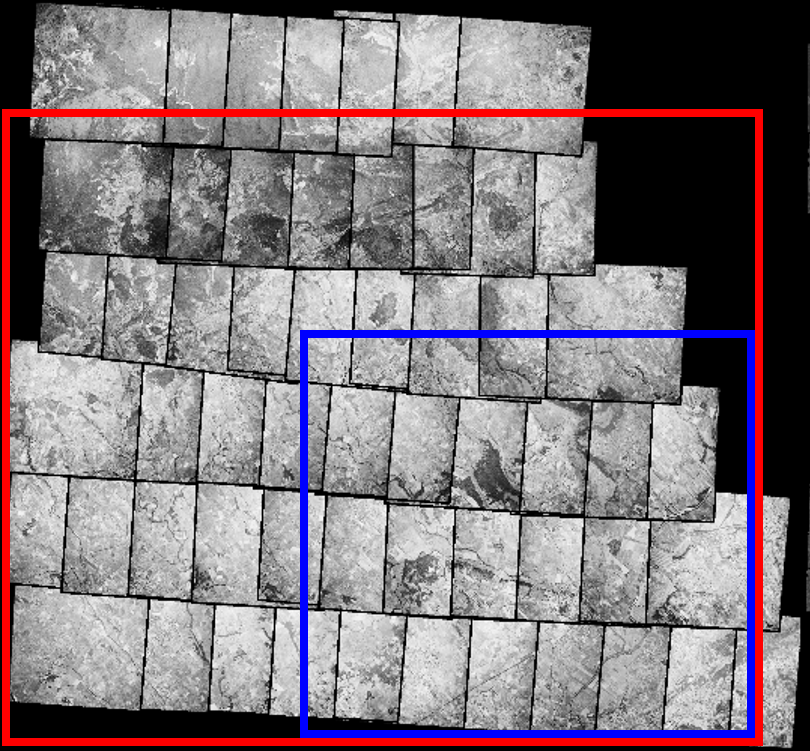
\includegraphics[width=6.45cm]{images/Chapitre3/Pezenas1971.png}
            \end{minipage}%
        }
        \subfigure[Pezenas 1981 (27 images)]{
            \begin{minipage}[t]{0.48\linewidth}
                \centering
                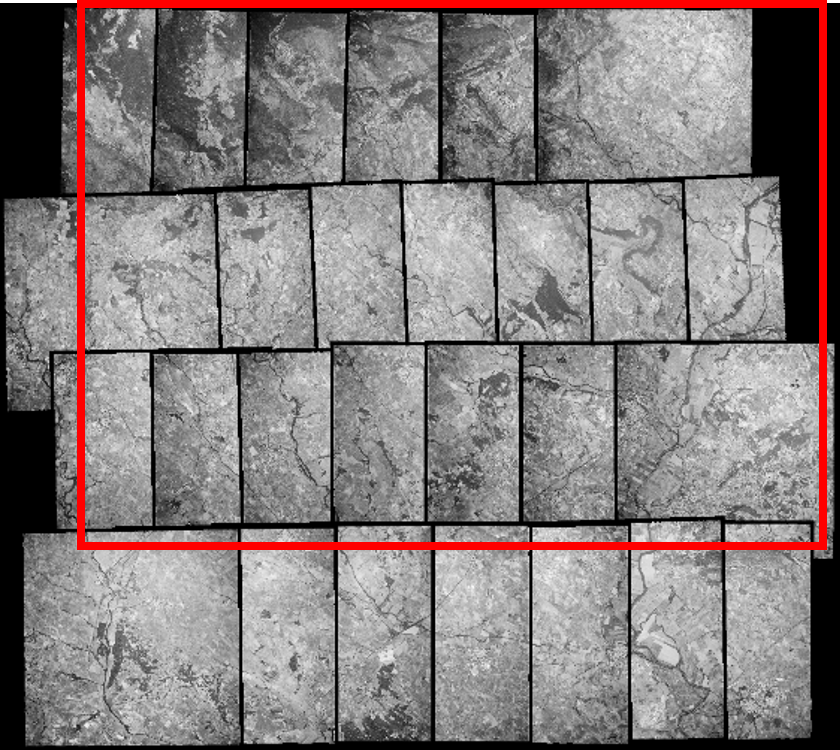
\includegraphics[width=6.68cm]{images/Chapitre3/Pezenas1981.png}
            \end{minipage}%
        }
            \subfigure[Pezenas 2014 (2 satellite images)]{
    	\begin{minipage}[t]{0.48\linewidth}
    		\centering
    		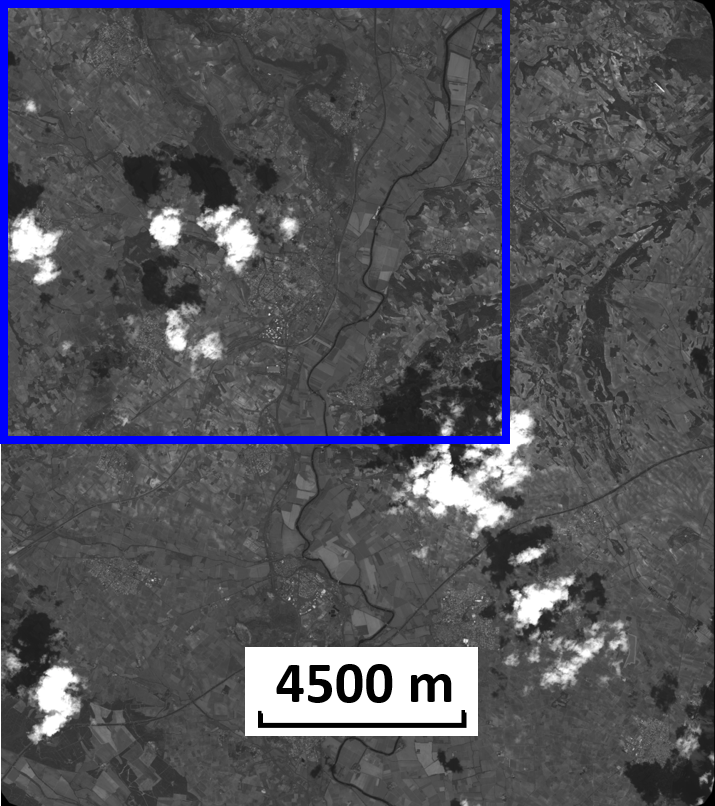
\includegraphics[width=6.6cm]{images/Chapitre3/Pezenas2014.png}
    	\end{minipage}%
    }
        \subfigure[Pezenas 2015 (382 images)]{
            \begin{minipage}[t]{0.48\linewidth}
                \centering
                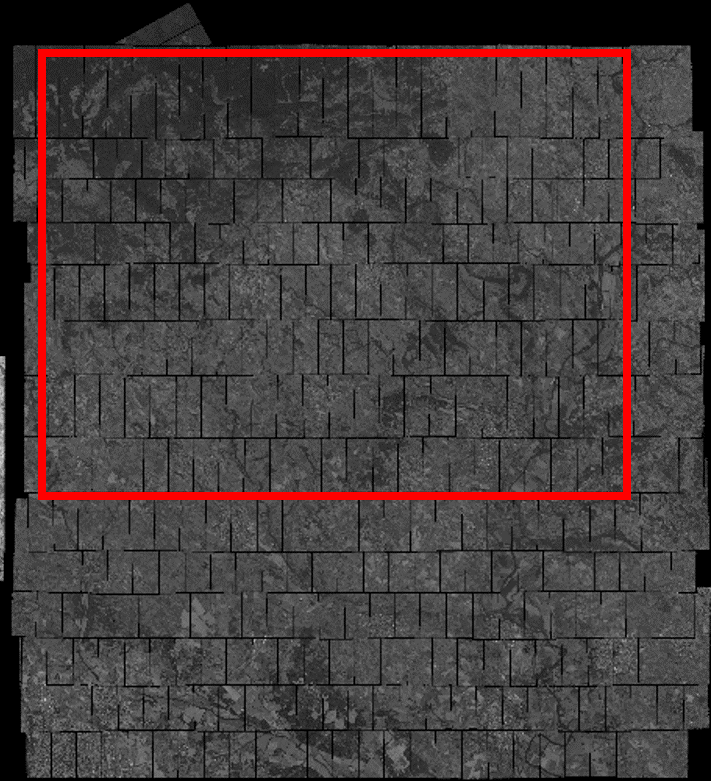
\includegraphics[width=6.78cm]{images/Chapitre3/Pezenas2015.png}
            \end{minipage}%
        }
        \caption{Images demonstration of different aerial epochs as well as satellite epoch in \textbf{Pezenas}, image number of each epoch is displayed in the parenthesis of each sub headline. There are 2 historical aerial epochs (1971 and 1981) and 2 \ac{GT} epochs (2014 the satellite epoch and 2015 the aerial epoch) in this dataset. The common zone between the historical epochs and the 2014 satellite epoch is indicated by the blue rectangles, while that between historical epochs and the 2015 aerial epoch is in red rectangles. Graphic scales are demonstrated on epoch 2014 and 2015 in (c) and (d).}
        \label{PezenasData}
    \end{center}
\end{figure*} 


\begin{figure*}[htbp]
    \begin{center}
        \subfigure[Kobe 1991 (15 images)]{
            \begin{minipage}[t]{1\linewidth}
                \centering
                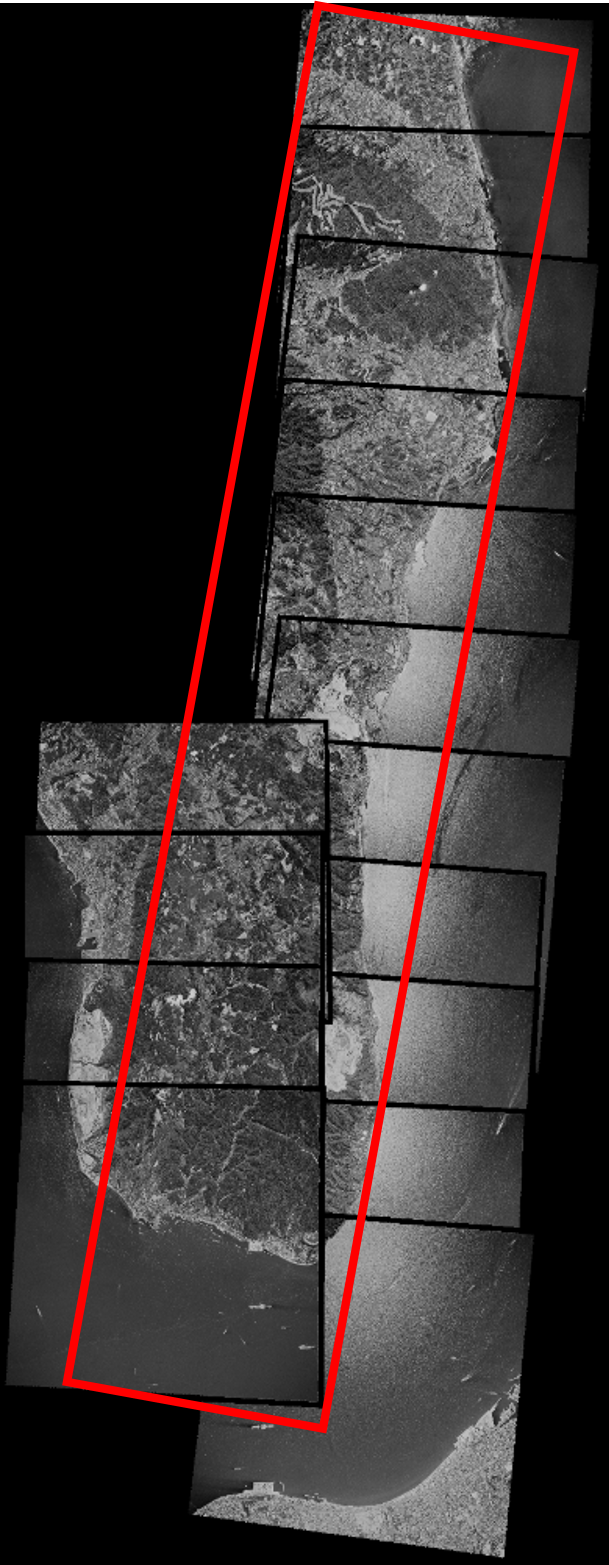
\includegraphics[height=13cm,angle=90]{images/Chapitre3/Kobe1991.png}
            \end{minipage}%
        }
        \subfigure[Kobe 1995 (83 images)]{
            \begin{minipage}[t]{1\linewidth}
                \centering
                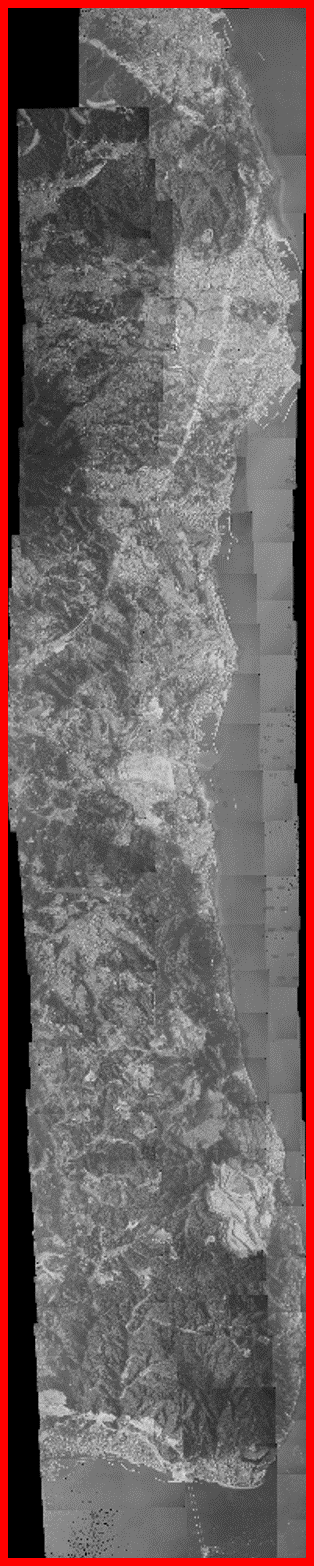
\includegraphics[height=13cm,angle=90]{images/Chapitre3/Kobe1995.png}
            \end{minipage}%
        }
        \caption{Images demonstration of different aerial epochs in \textbf{Kobe}, image number of each epoch is displayed in the parenthesis of each sub headline. The common zone between all the epochs is indicated by the red rectangles. Graphic scale is demonstrated on epoch 1995 in (b).}
        \label{KobeData}
    \end{center}
\end{figure*} 

\begin{figure*}[htbp]
	\begin{center}
		\subfigure[Alberona 1954 (3 images)]{
			\begin{minipage}[t]{0.48\linewidth}
				\centering
				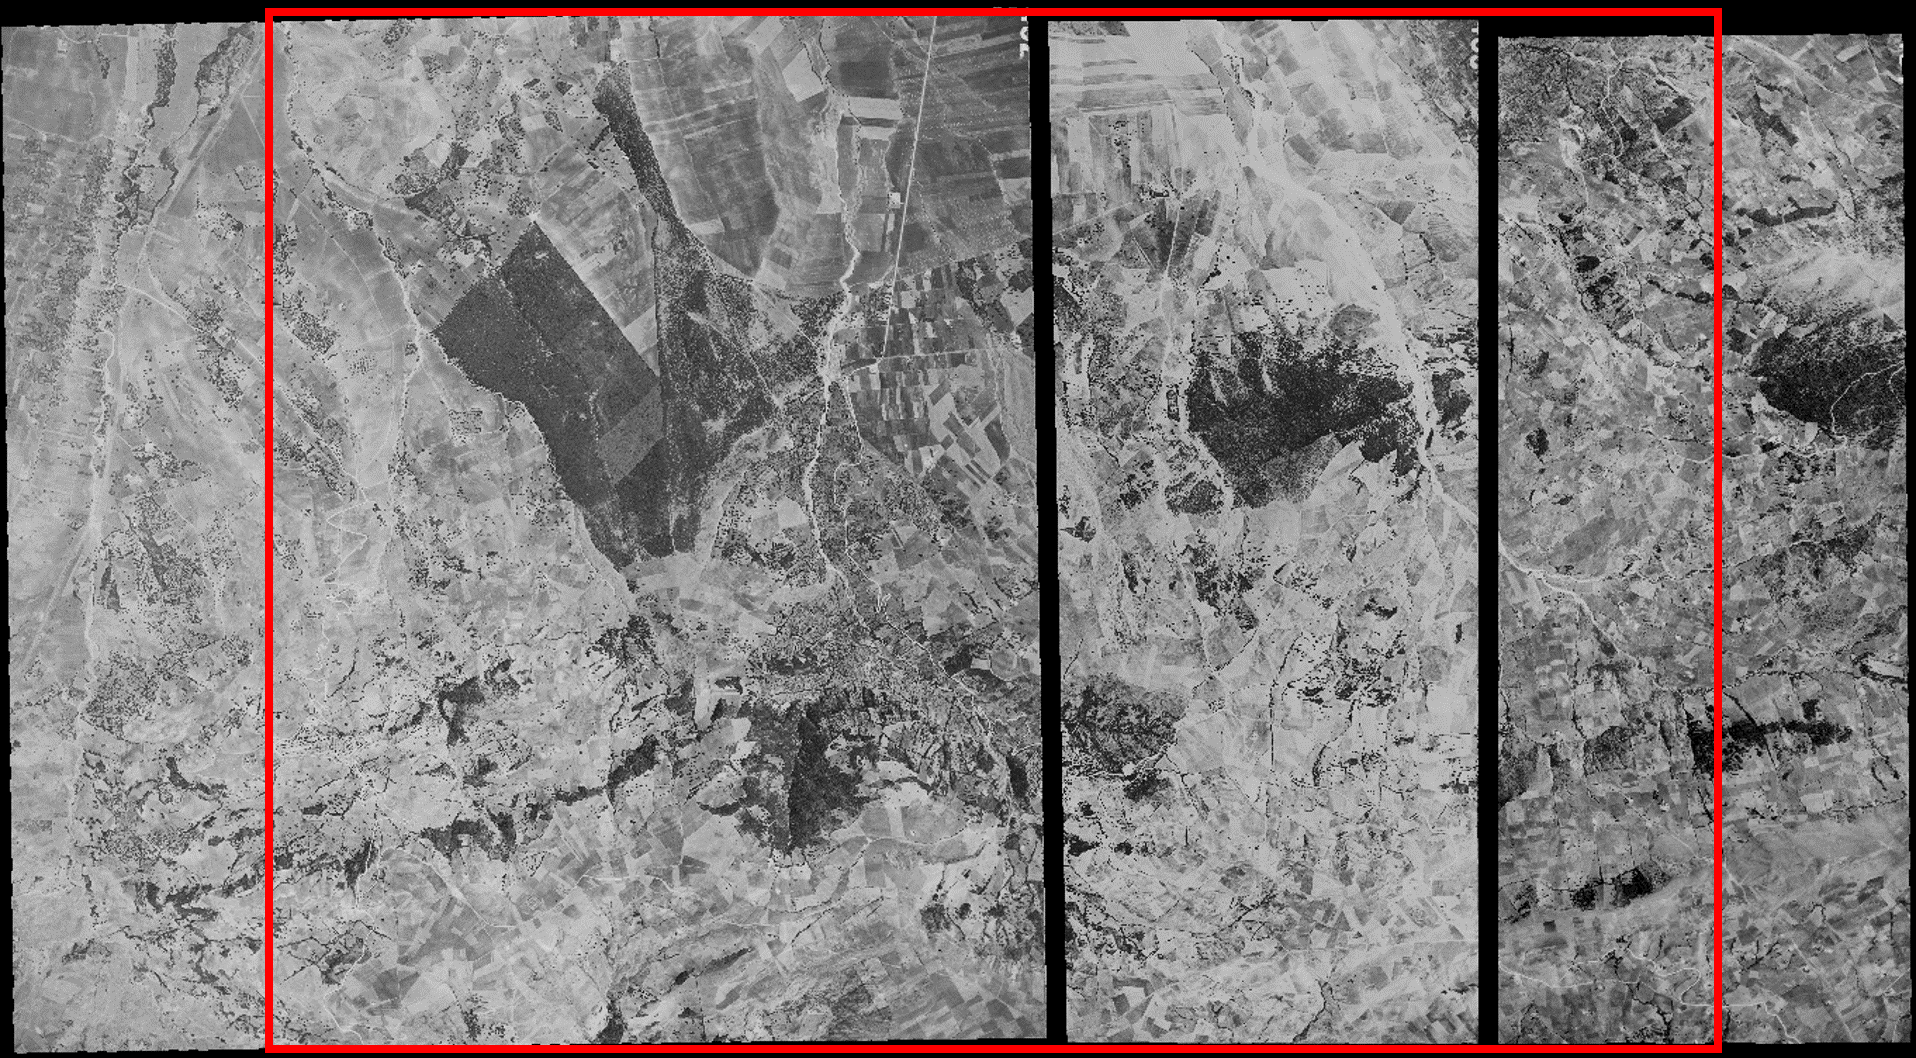
\includegraphics[width=6.2cm]{images/ChapitreNew/Ortho-MEC-Malt_Tapas_1954.png}
			\end{minipage}%
		}
		\subfigure[Alberona 2003 (7 images)]{
			\begin{minipage}[t]{0.48\linewidth}
				\centering
				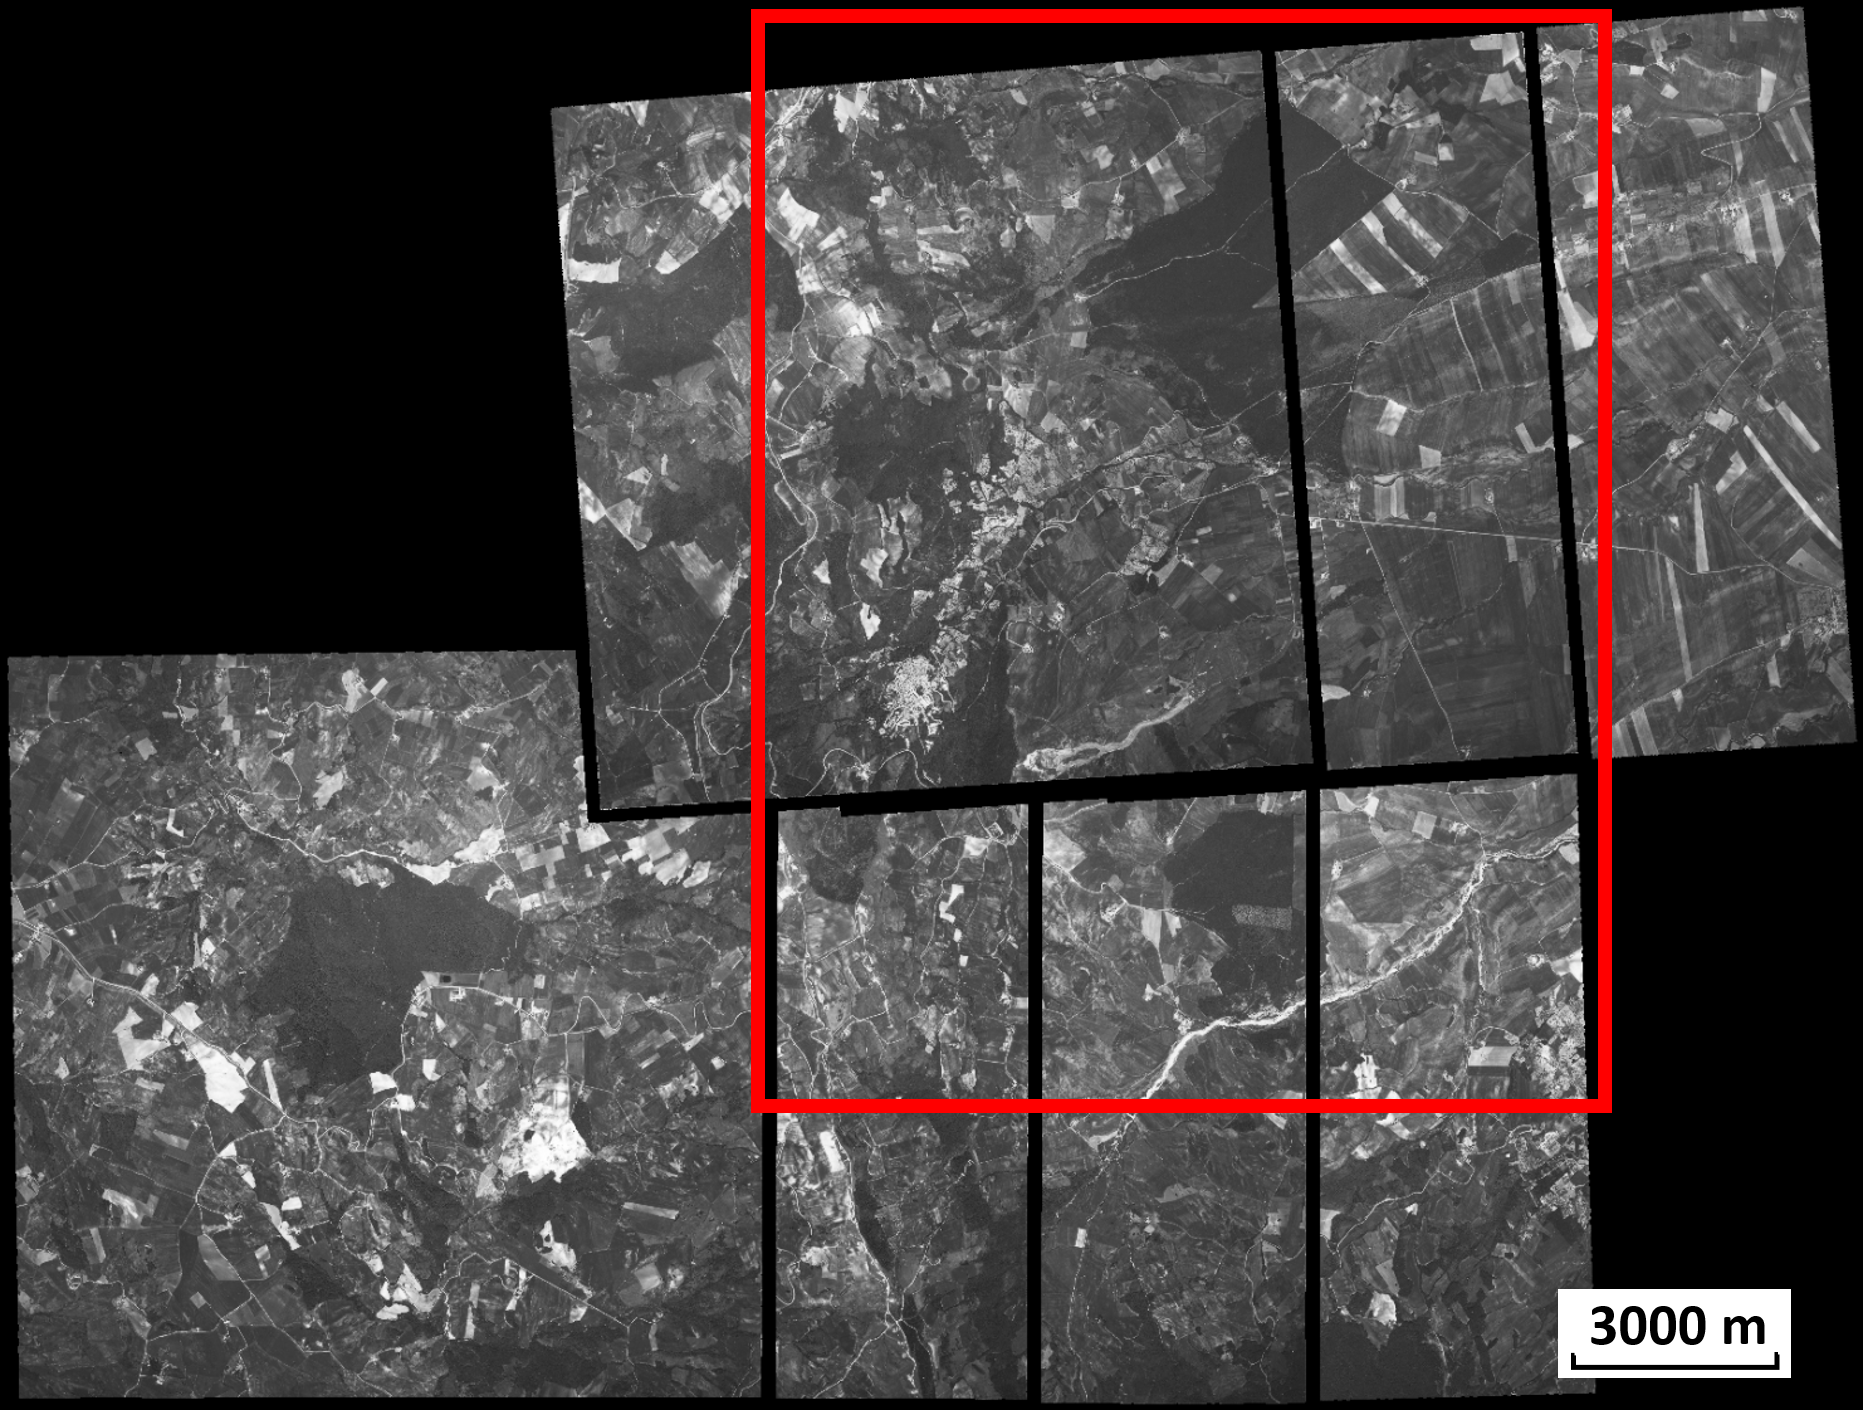
\includegraphics[width=6.2cm]{images/ChapitreNew/Ortho-MEC-Malt_Tapas_2003.png}
			\end{minipage}%
		}
		\caption{Images demonstration of different aerial epochs in \textbf{Alberona}, image number of each epoch is displayed in the parenthesis of each sub headline. The common zone between all the epochs is indicated by the red rectangles. Graphic scale is demonstrated on epoch 2003 in (b).}
		\label{AlberonaData}
	\end{center}
\end{figure*} 

\begin{figure*}[htbp]
	\begin{center}
		\subfigure[Image 1]{
			\begin{minipage}[t]{0.31\linewidth}
				\centering
				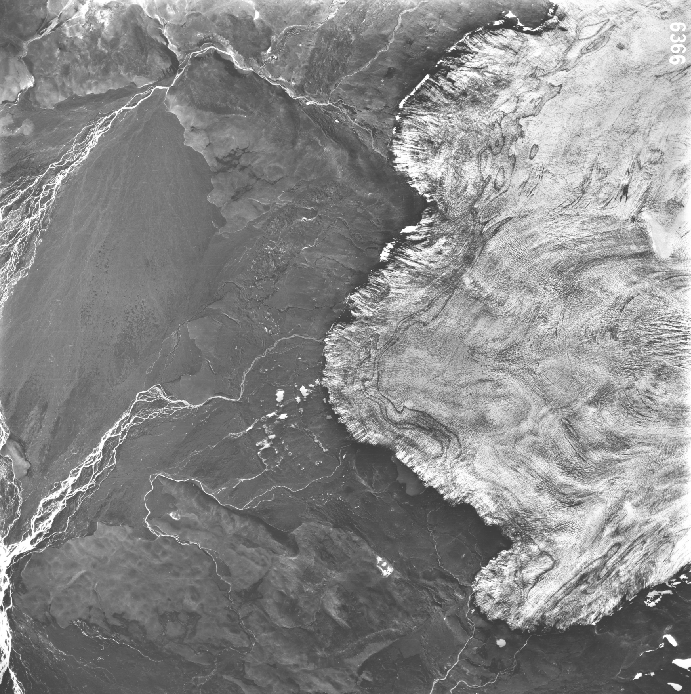
\includegraphics[width=4.3cm]{images/ChapitreNew/3-6366_crp_8Bits_Zoom8.png}
			\end{minipage}%
		}
		\subfigure[Image 2]{
			\begin{minipage}[t]{0.31\linewidth}
				\centering
				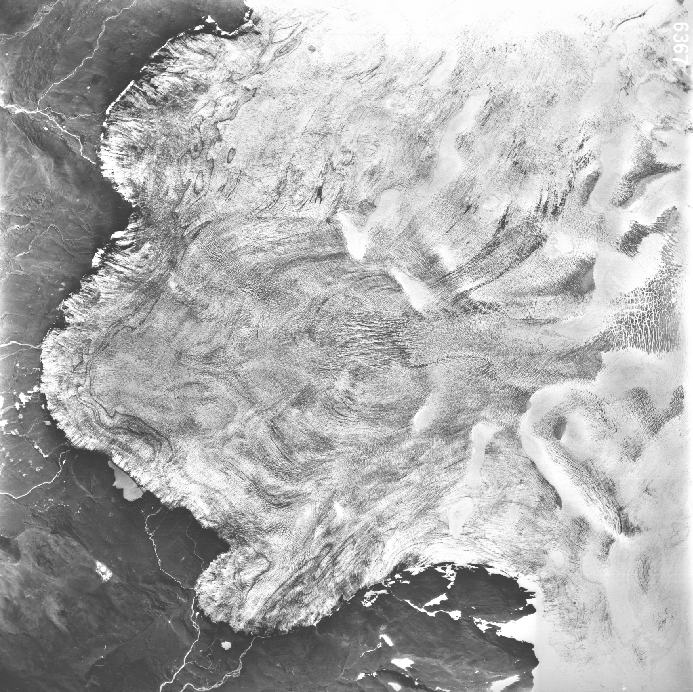
\includegraphics[width=4.3cm]{images/ChapitreNew/3-6367_crp_8Bits_Zoom8.png}
			\end{minipage}%
		}
		\subfigure[Image 3]{
			\begin{minipage}[t]{0.31\linewidth}
				\centering
				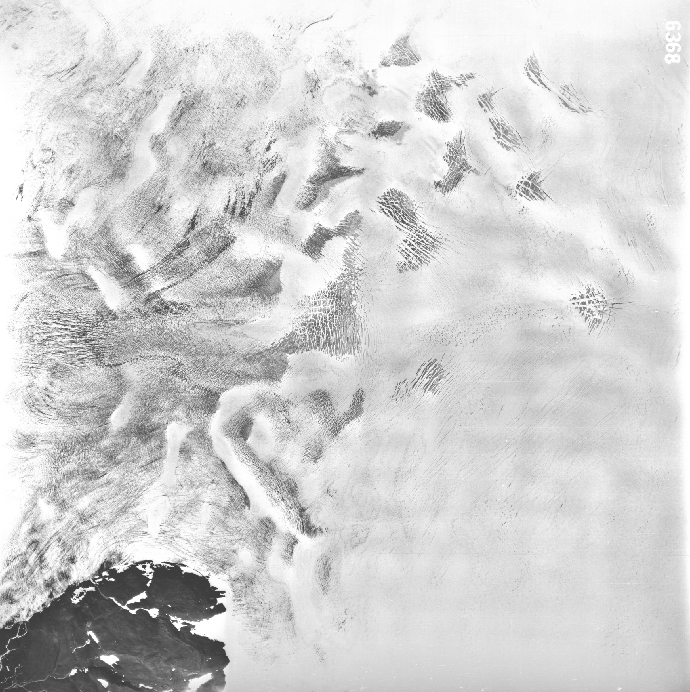
\includegraphics[width=4.3cm]{images/ChapitreNew/3-6368_crp_8Bits_Zoom8.png}
			\end{minipage}%
		}
		\subfigure[Image 4]{
			\begin{minipage}[t]{0.31\linewidth}
				\centering
				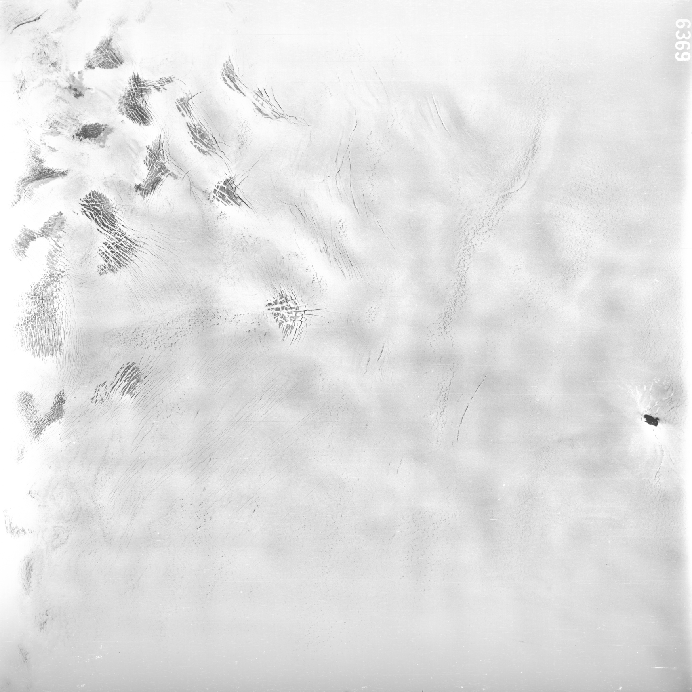
\includegraphics[width=4.3cm]{images/ChapitreNew/3-6369_crp_8Bits_Zoom8.png}
			\end{minipage}%
		}
		\subfigure[Image 5]{
			\begin{minipage}[t]{0.31\linewidth}
				\centering
				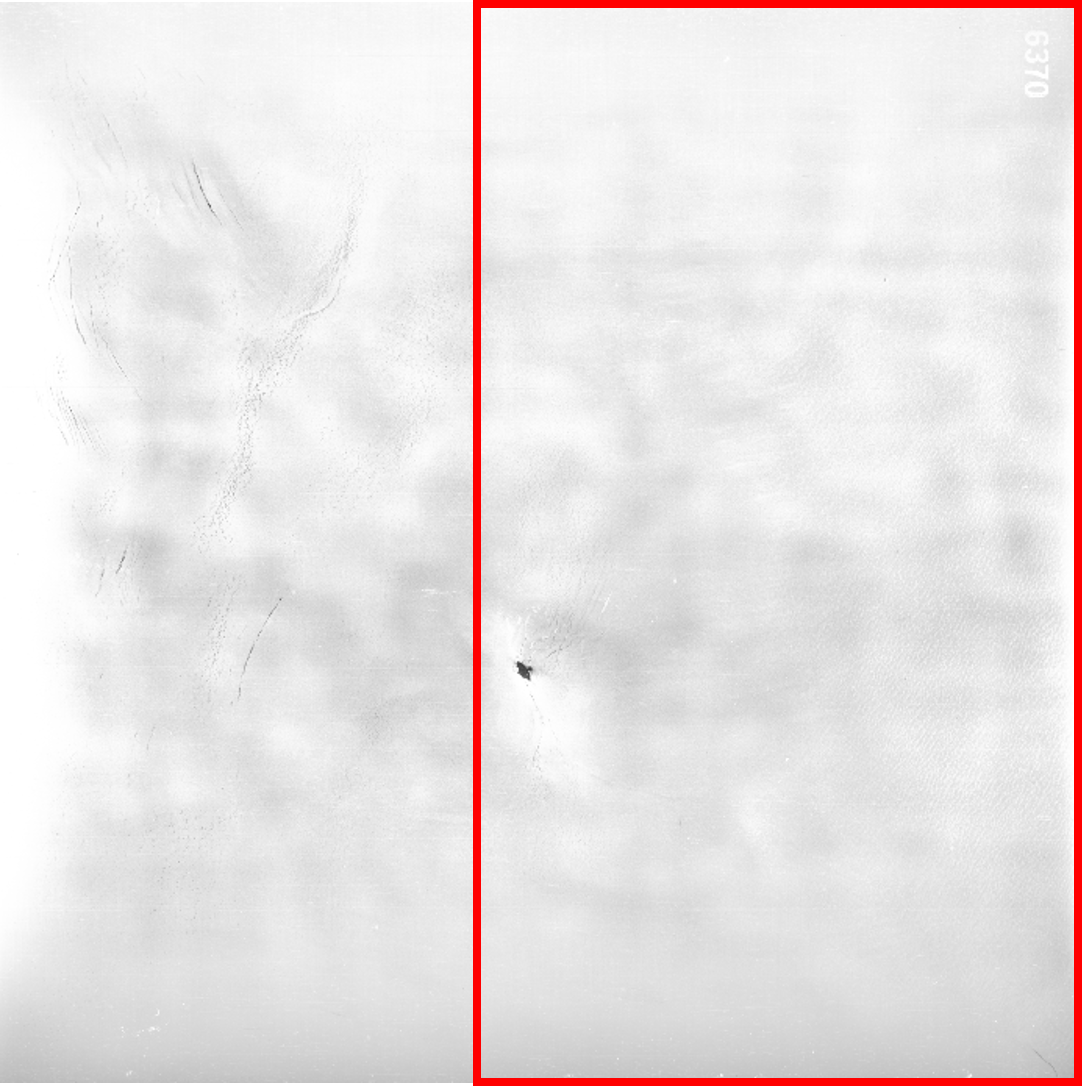
\includegraphics[width=4.3cm]{images/ChapitreNew/3-6370_crp_8Bits_Zoom8.png}
			\end{minipage}%
		}
		\subfigure[Image 6]{
			\begin{minipage}[t]{0.31\linewidth}
				\centering
				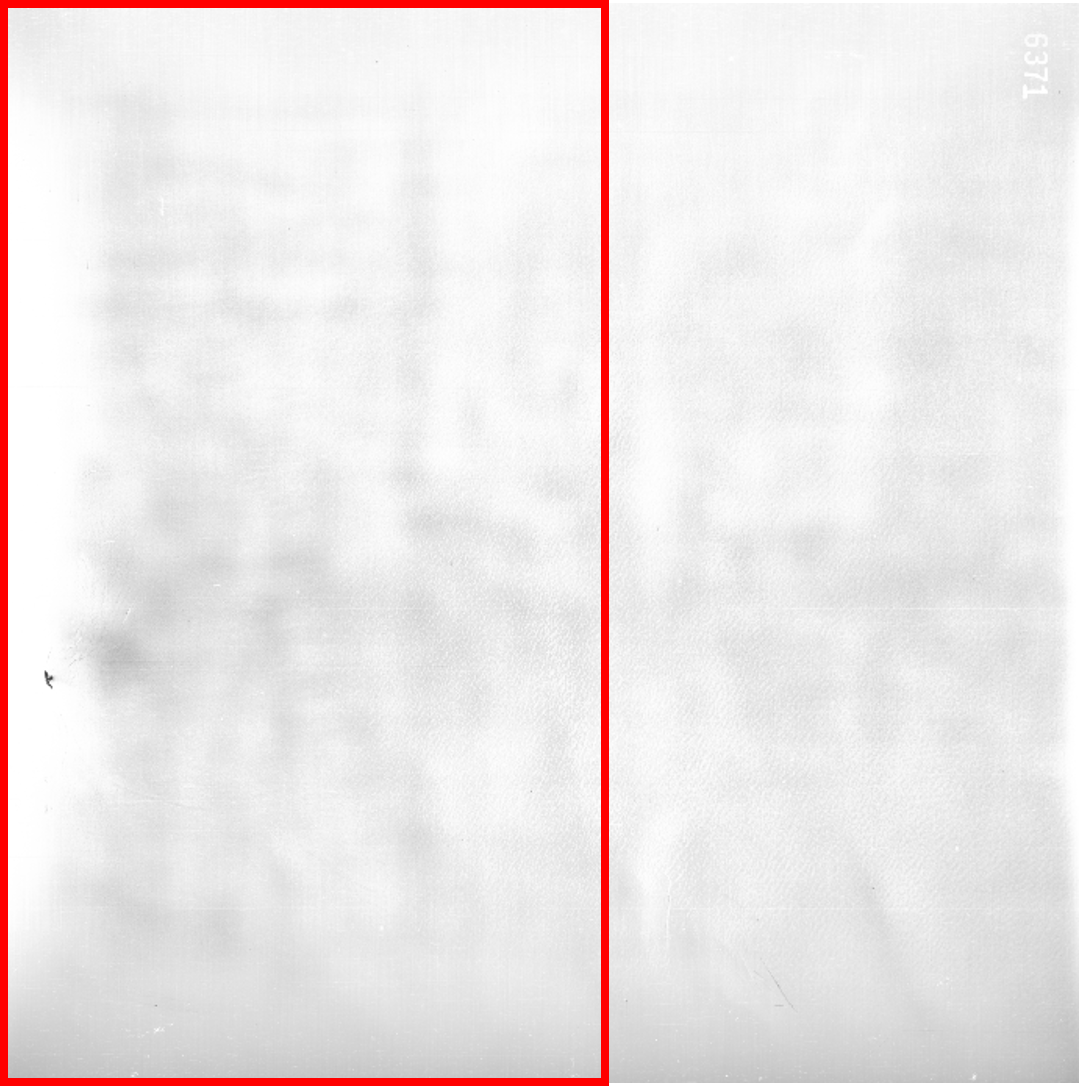
\includegraphics[width=4.3cm]{images/ChapitreNew/3-6371_crp_8Bits_Zoom8.png}
			\end{minipage}%
		}
		\caption{Images demonstration of epoch 1960 in \textbf{Hofsjökull}.}
		\label{Hofsjökull}
	\end{center}
\end{figure*} 
